\documentclass[aspectratio=169]{beamer}
\usepackage{amsmath, amssymb, amsfonts, amsthm}
\usepackage{cancel}
\usepackage[output-complex-root=j]{siunitx}
\usepackage[american, nooldvoltagedirection]{circuitikz}
\usepackage{bm}
\usepackage{listings}
\usepackage{graphicx}
\usepackage{hyperref}

\usetheme{Berkeley}
\usefonttheme[onlymath]{serif}
\AtBeginSection[]{
    \begin{frame}
    \vfill
    \centering
    \begin{beamercolorbox}[sep=8pt,center,shadow=false,rounded=false]{title}
        \usebeamerfont{title}\insertsectionhead\par
    \end{beamercolorbox}
    \vfill
    \end{frame}
}

\newcommand{\N}{\mathbb{N}}
\newcommand{\Z}{\mathbb{Z}}
\newcommand{\Q}{\mathbb{Q}}
\newcommand{\R}{\mathbb{R}}
\renewcommand{\C}{\mathbb{C}}
\newcommand{\unit}[1]{\bm{\hat{#1}}}
\newcommand{\iprod}[2]{\left\langle #1, #2 \right\rangle}
\newcommand{\tpose}[1]{\left[#1\right]^{\! \top} \!\!}
\newcommand{\diff}[1]{\frac{d}{d #1}}

\title{EECS 16B CSM}
\author{Bryan Ngo}
\date{2020-09-14}
\institute{Computer Science Mentors}

\begin{document}

\begin{frame}
    \maketitle
\end{frame}

\begin{frame}
    \frametitle{Who am I?}

    \begin{columns}
        \column[]{0.5\textwidth}
        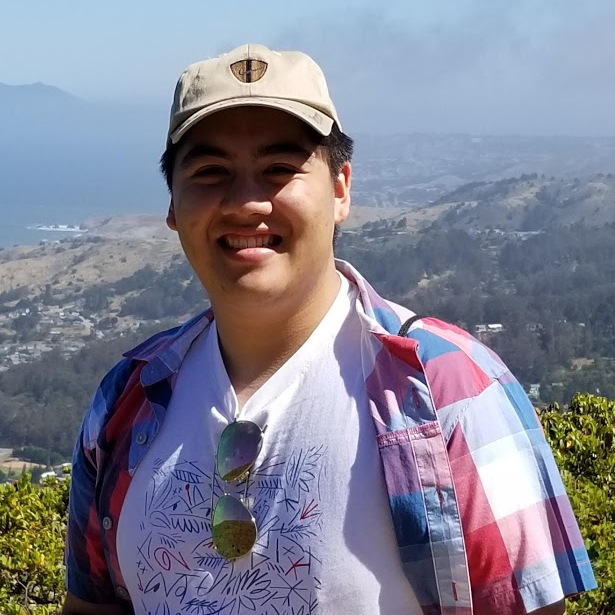
\includegraphics[width=0.8\textheight]{bryan_ngo.png}

        \column[]{0.5\textwidth}
        \begin{itemize}
            \item 2nd year majoring in EECS
            \item first time in CSM!
            \item took EECS 16B Spring 2020
            \item How I spent quarantine
            \begin{itemize}
                \item lots of vidya (Hitman 2, Civ VI, Stellaris, etc.)
                \item learned Haskell
                \item building mechanical keyboard
            \end{itemize}
        \end{itemize}
    \end{columns}
\end{frame}

\begin{frame}
    \frametitle{Who are you?}

    \begin{itemize}
        \item Name
        \item Major
        \item How you spent quarantine
        \item Most mundane/interesting fact about yourself
    \end{itemize}
\end{frame}

\begin{frame}
    \frametitle{Logistics}

    \begin{itemize}
        \item Join \href{http://piazza.com/berkeley/fall2020/csm16b}{Piazza}
        \item unexcused absences in first 3 weeks \(\to\) \textbf{auto-dropped \& NP}
        \item excused absences
        \begin{itemize}
            \item email \href{mailto:bryanngo@berkeley.edu}{bryanngo@berkeley.edu} \& cc \href{mailto:mentors@berkeley.edu}{mentors@berkeley.edu} with subject line \texttt{[Request for Absence] <course>}
        \end{itemize}
    \end{itemize}
\end{frame}

\begin{frame}
    \frametitle{Expectations}
    \framesubtitle{Me to You}

    \begin{itemize}
        \item Be skeptical
        \item Constant feedback
        \item Become passionate about 16B
    \end{itemize}
\end{frame}

\begin{frame}
    \frametitle{Expectations}
    \framesubtitle{You to Me}

    \begin{itemize}
        \item Lecture:worksheet ratio?
        \item Get a webcam?
        \item Stop typing so loud?
    \end{itemize}
\end{frame}

\section{Differential Equations}

\begin{frame}
    \frametitle{The Derivative}

    \begin{equation}
        \diff{x} f(x) = \lim_{h \to 0} \frac{f(x + h) - f(x)}{h}
    \end{equation}
    \begin{itemize}
        \item describes instantaneous rate of change
    \end{itemize}
\end{frame}

\begin{frame}
    \frametitle{Differential Equations}

    \begin{itemize}
        \item \href{https://youtu.be/p_di4Zn4wz4?list=PLZHQObOWTQDNPOjrT6KVlfJuKtYTftqH6}{3Blue1Brown video}
    \end{itemize}

\end{frame}

\end{document}
